% This LaTeX was auto-generated from MATLAB code.
% To make changes, update the MATLAB code and export to LaTeX again.

\documentclass{article}

\usepackage[utf8]{inputenc}
\usepackage[T1]{fontenc}
\usepackage{lmodern}
\usepackage{graphicx}
\usepackage{color}
\usepackage{hyperref}
\usepackage{amsmath}
\usepackage{amsfonts}
\usepackage{epstopdf}
\usepackage[table]{xcolor}
\usepackage{matlab}
\usepackage[paperheight=845pt,paperwidth=597pt,top=85pt,bottom=85pt,right=85pt,left=85pt,heightrounded]{geometry}

\sloppy
\epstopdfsetup{outdir=./}
\graphicspath{ {./analisiPrestazionale_media/} }

\begin{document}


\begin{matlabcode}
b = sum(A,2);
x = ones(N,1);

[xJM1,flagJM1,relresJM1,iterJM1,resvecJM1] = jacobi(A,b);
% Calcolo dell'errore assoluto

% Rappresentazione grafica errore assoluto
figure(1)
semilogy(errJM1, 'o');
ylabel('Errore $\mathbf{e}_{abs}^{(k)}$', 'Interpreter','latex','FontSize',12);
xlabel('Componente $x_{i}$', 'Interpreter','latex','FontSize',12);
\end{matlabcode}
\begin{center}
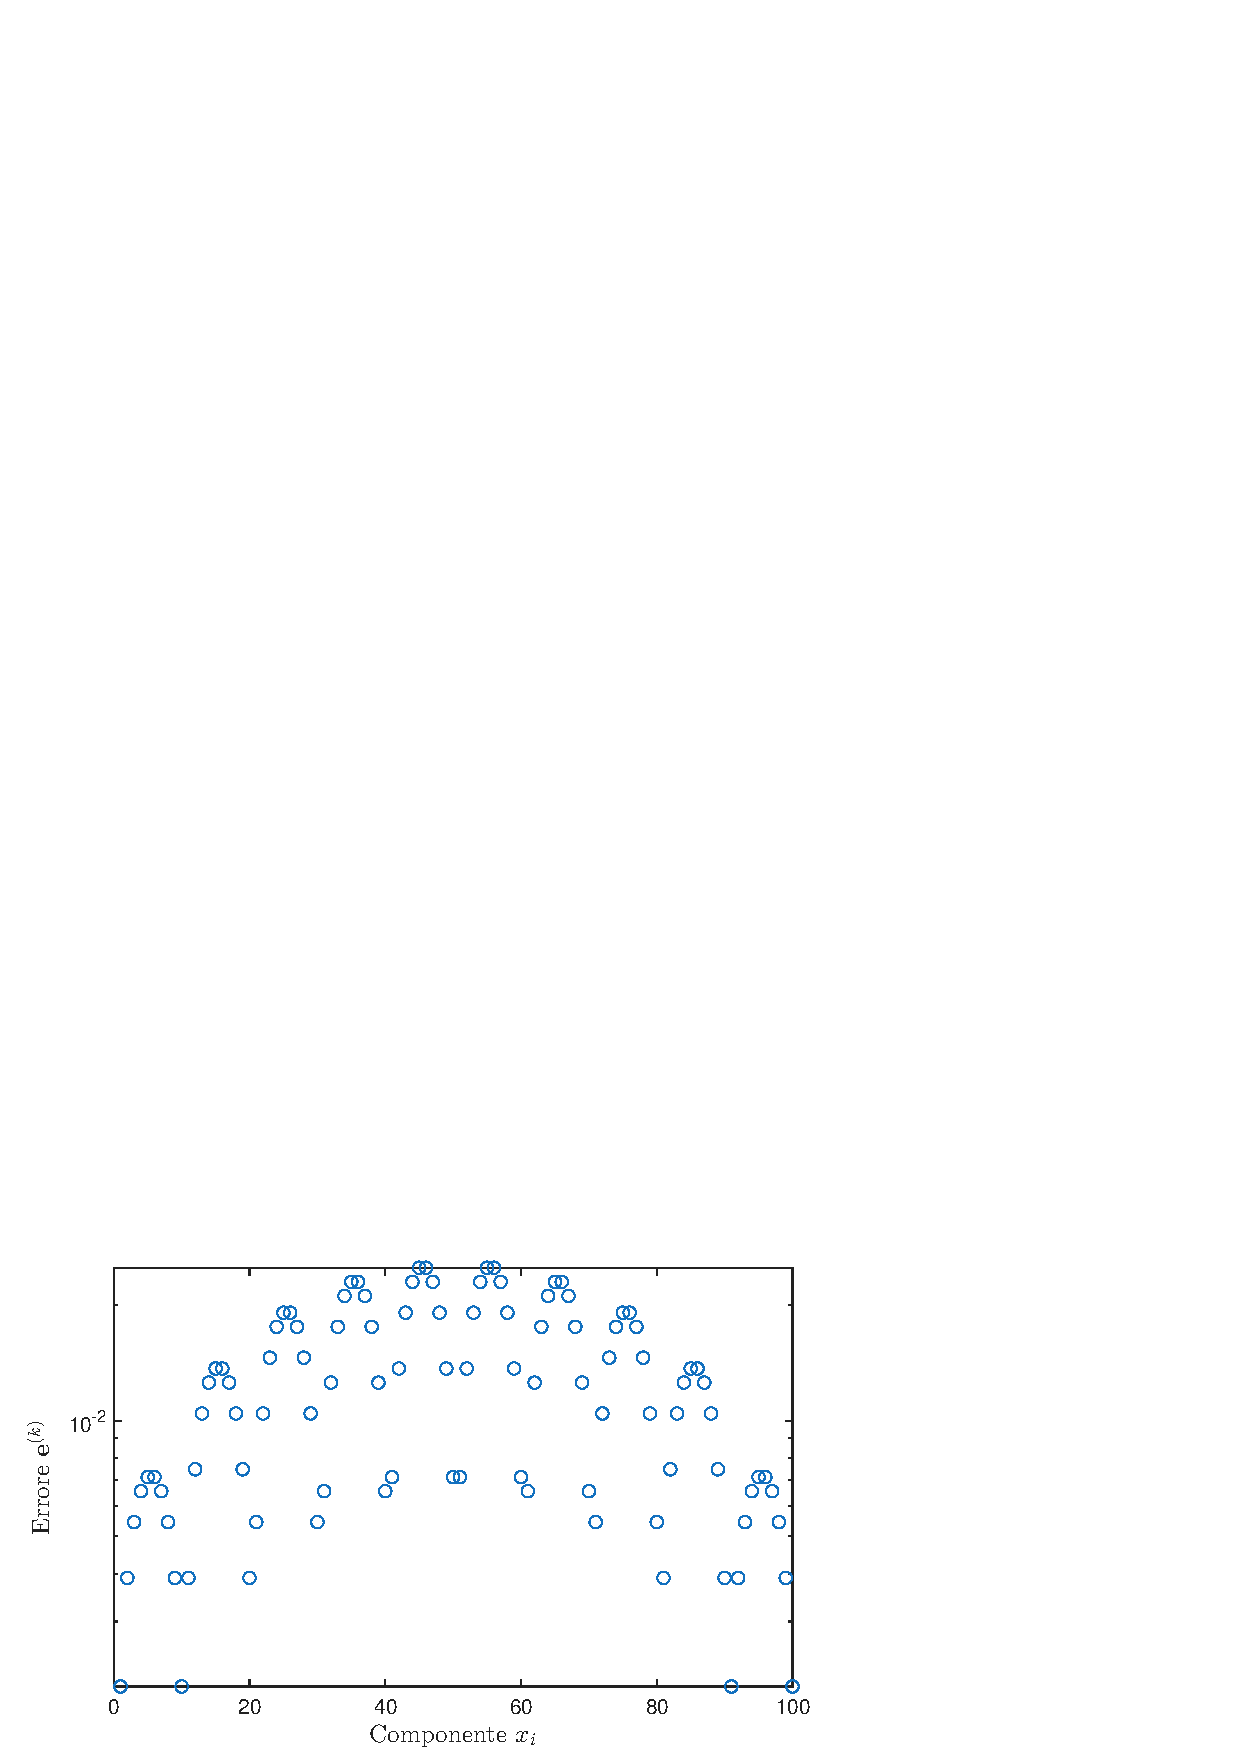
\includegraphics[width=\maxwidth{56.196688409433015em}]{figure_0.png}
\end{center}
\begin{matlabcode}
if flagJM1 == 1
fprintf("jacobi si è fermato all'iterazione numero %u senza " + ...
        "raggiungere la tolleranza desiderata %0.2g\n" + ...
        "poiché il numero massimo di iterazioni %u " + ...
        "è stato raggiunto.\nL'ultima iterazione presenta residuo relativo pari a %0.2g.\n", ...
        iterJM1, 1e-6, 100, relresJM1);
end
\end{matlabcode}
\begin{matlaboutput}
jacobi si è fermato all'iterazione numero 100 senza raggiungere la tolleranza desiderata 1e-06
poiché il numero massimo di iterazioni 100 è stato raggiunto.
L'ultima iterazione presenta residuo relativo pari a 0.028.
\end{matlaboutput}
\begin{matlabcode}
maxit = 3e5;

tJM2 = tic;
[xJM2,flagJM2,relresJM2,iterJM2,resvecJM2] = jacobi(A,b,[],maxit);
tJM2 = toc(tJM2);

if flagJM2 == 0
     fprintf("jacobi ha raggiunto la convergenza all'iterazione %u, calcolando " + ...
             "una soluzione approssimata avente residuo relativo\npari a %0.2g.\n",iterJM2,relresJM2);
    xJM2par = xJM2(1:10)
     fprintf("Tempo di esecuzione per il metodo di Jacobi: %f sec.", tJM2);
end
\end{matlabcode}
\begin{matlaboutput}
jacobi ha raggiunto la convergenza all'iterazione 210137, calcolando una soluzione approssimata avente residuo relativo
pari a 1e-06.
xJM2par = 10x1
    1.0000
    1.0000
    1.0000
    1.0000
    1.0000
    1.0000
    1.0000
    1.0000
    1.0000
    1.0000

Tempo di esecuzione per il metodo di Jacobi: 437.693564 sec.
\end{matlaboutput}
\begin{matlabcode}
errJM2 = abs(x - xJM2);

figure(2)
semilogy(errJM1,'o');
hold on
semilogy(errJM2,'diamond');
ylabel('Errore $\mathbf{e}_{abs}^{(k)}$', 'Interpreter','latex','FontSize',12);
xlabel('Componente $x_{i}$', 'Interpreter','latex','FontSize',12);
legend('$\texttt{maxit}=100$','$\texttt{maxit}=3\times10^{\text{3}}', 'Interpreter', 'latex');
hold off
\end{matlabcode}
\begin{center}
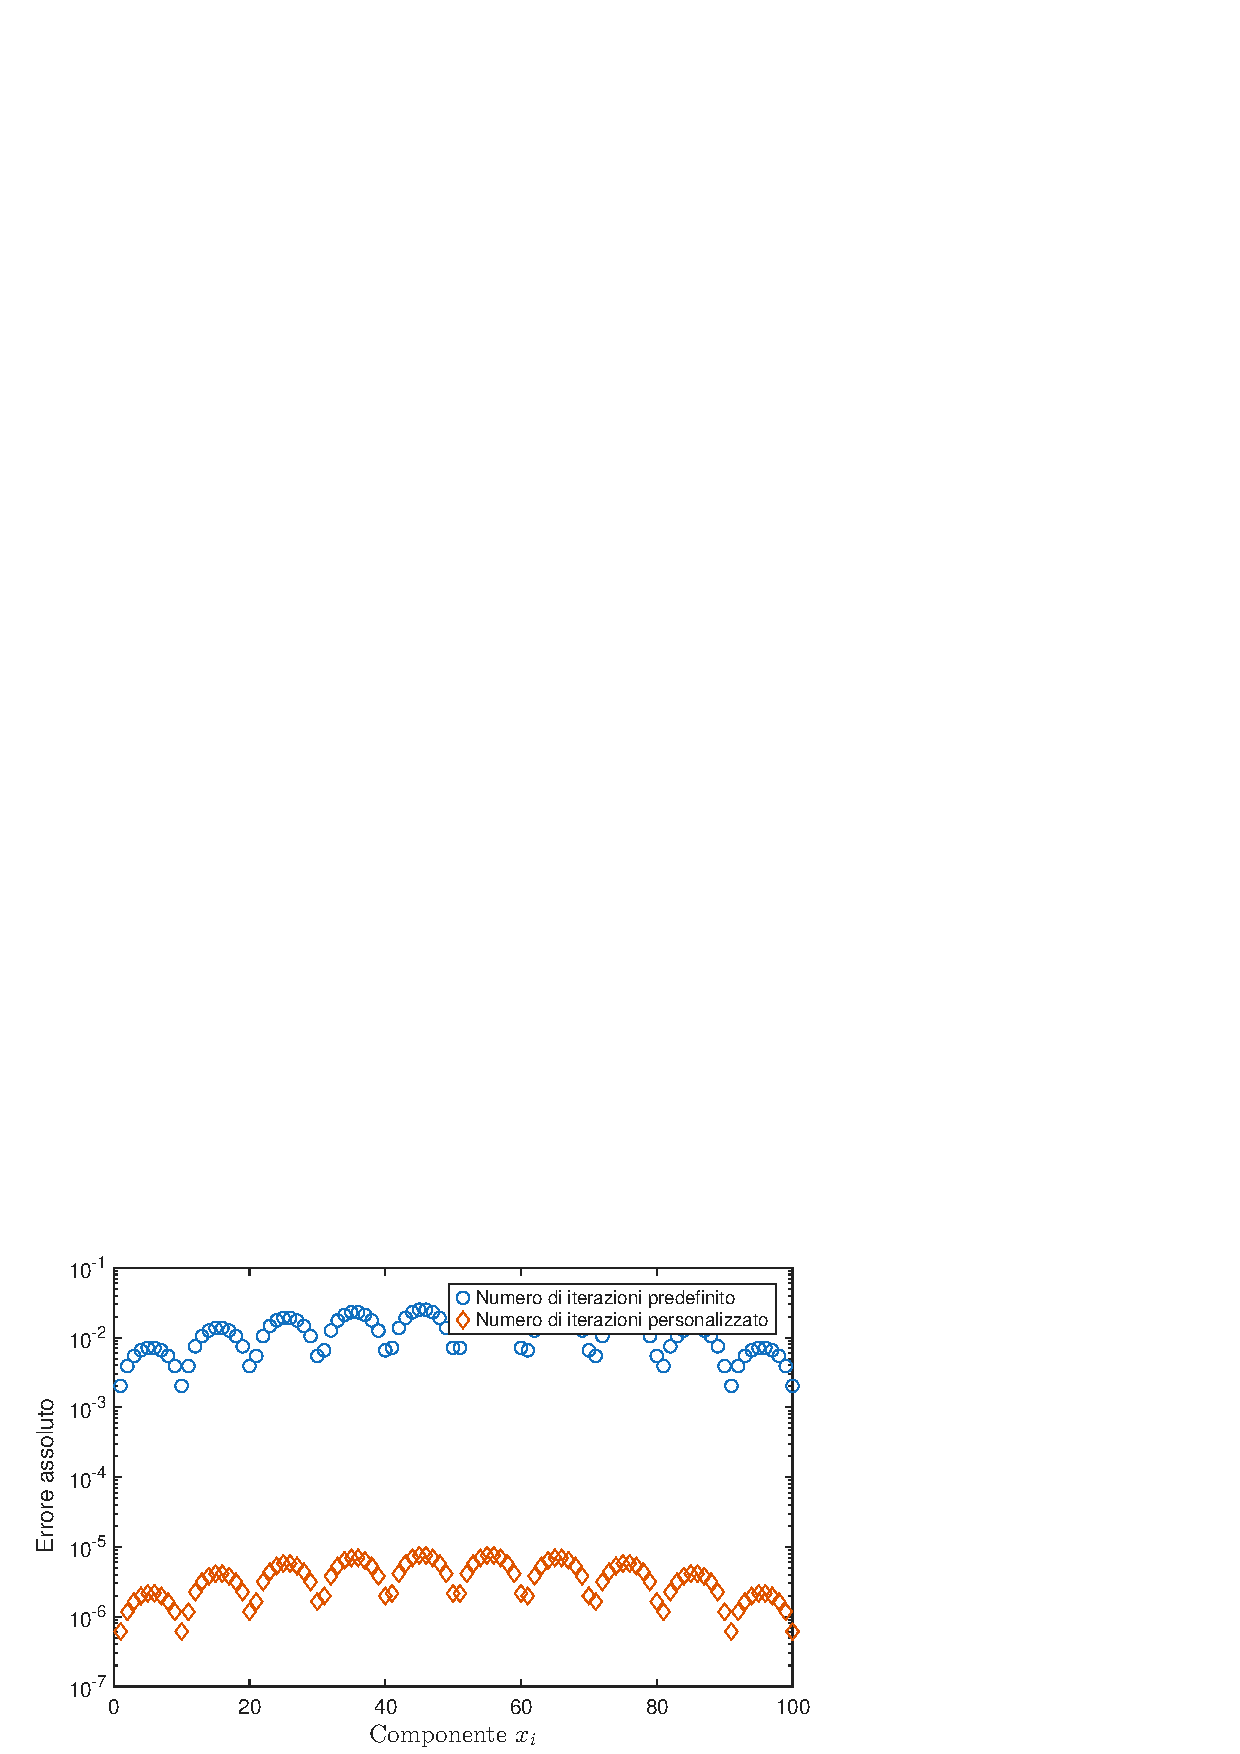
\includegraphics[width=\maxwidth{56.196688409433015em}]{figure_1.png}
\end{center}
\begin{matlabcode}
relresvecJM = resvecJM2./resvecJM2(1);

figure(3)
f=semilogy(relresvecJM);
hold on
semilogy(f.Parent.XLim,[1e-6 1e-6],'--')
semilogy([100 100], f.Parent.YLim,'--')

ylabel('Residuo relativo');
xlabel("Iterazioni");
legend('Residuo relativo','Tolleranza','Numero di iterazioni predefinito')
hold off
\end{matlabcode}
\begin{center}
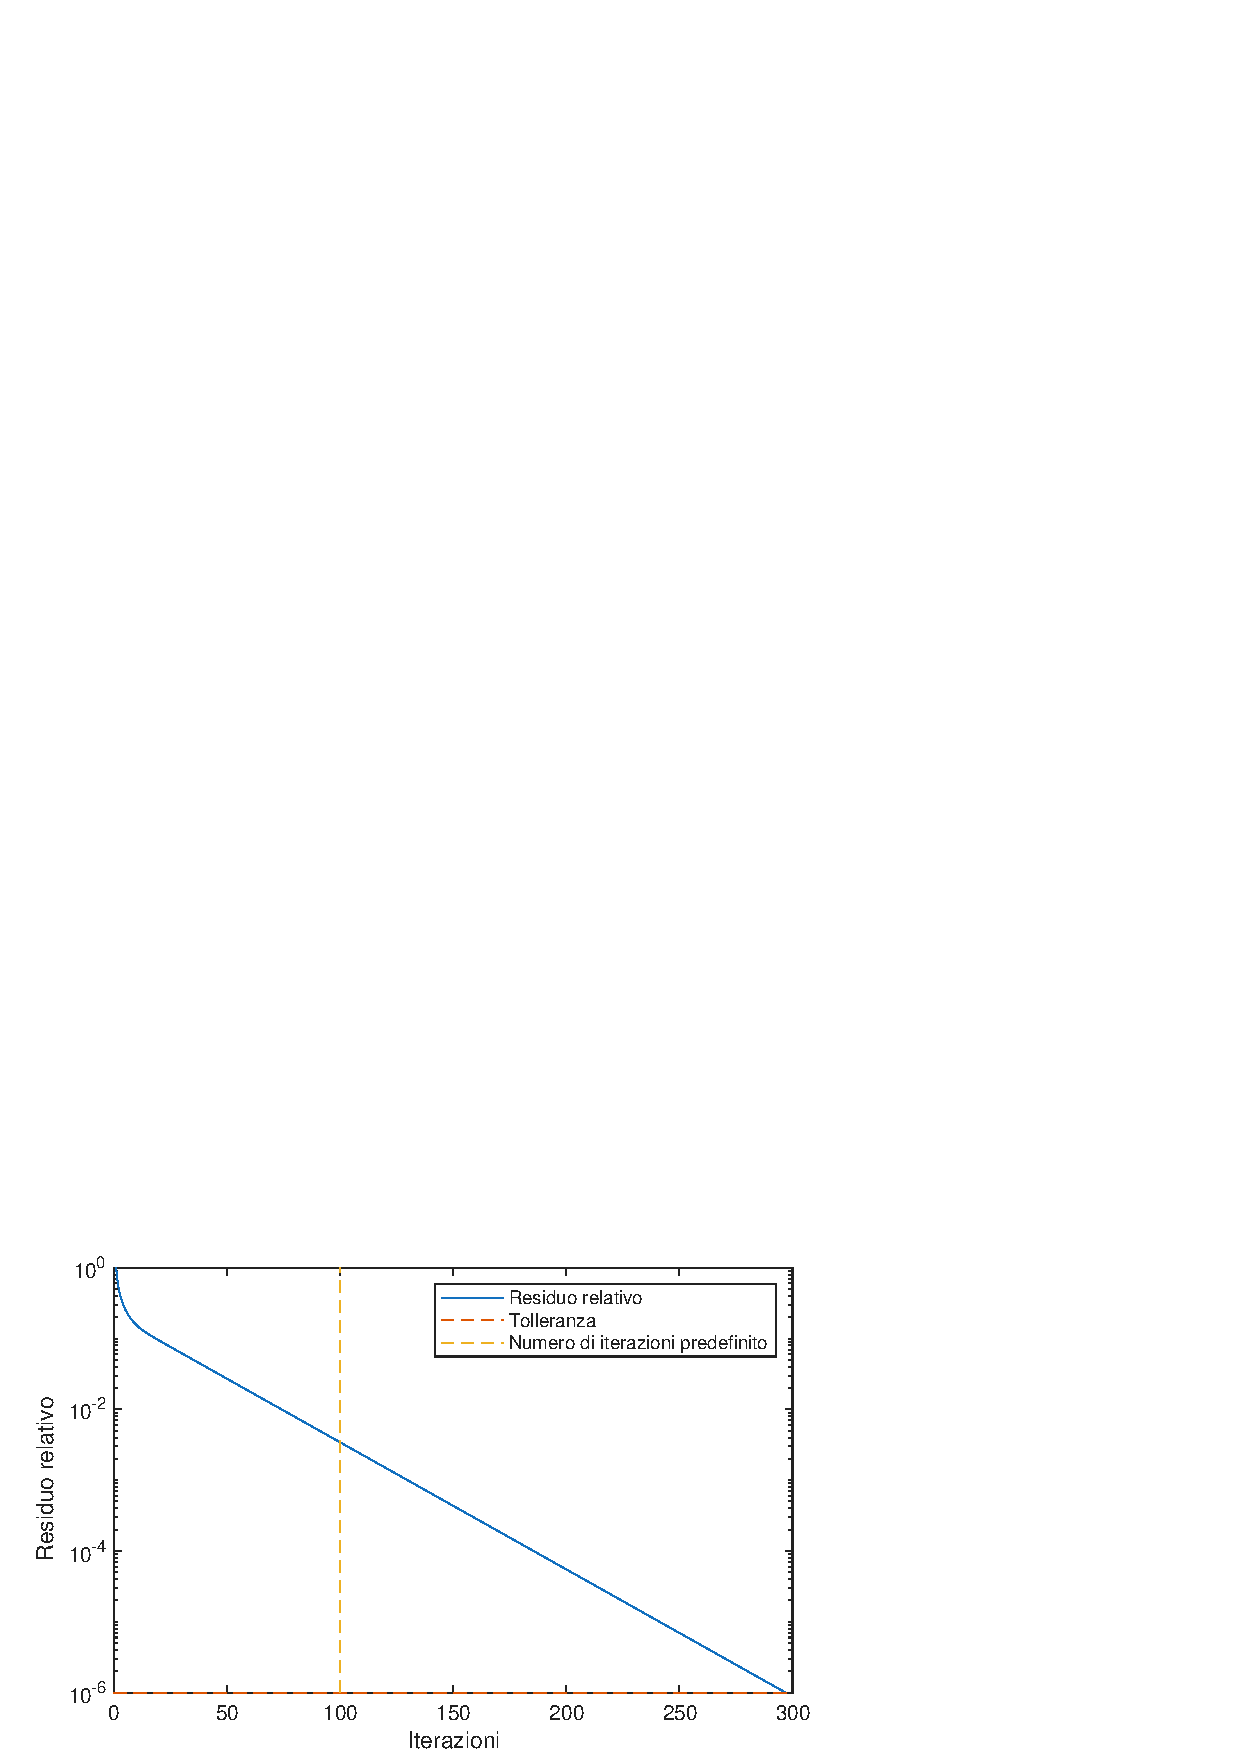
\includegraphics[width=\maxwidth{56.196688409433015em}]{figure_2.png}
\end{center}


\begin{matlabcode}
A = distributed((gallery('poisson', n)));
b = sum(A,2);
[xJM3,flagJM3,relresJM3,iterJM3,resvecJM3] = jacobi(A,b,[],maxit);
\end{matlabcode}

\end{document}
